\icode{E-MD-SI-L2-261119-002}
如图，质量分别为 \(2m\) 和 \(3m\) 的方形物体 \(A\) 和 \(B\) 在水平恒力 \(F\) 作用下，沿光滑水平面向右运动，\(A\) 刚好不下滑，设最大静摩擦力等于滑动摩擦力，重力加速度大小为 \(g\)，则 \(A\)、\(B\) 间的动摩擦因数为\paren[]
	
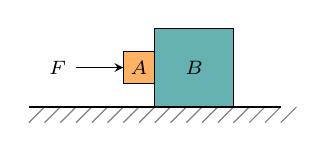
\begin{tikzpicture}[>=stealth,font=\scriptsize]
	\draw[fill=teal!60] (.4,0) rectangle(1.4,1)node[midway]{\(B\)};
	\draw[fill=orange!60] (0,.3) rectangle(.4,.7)node[midway]{\(A\)};
	\draw[->] (-.6,.5)node[left]{\(F\)}--(0,.5);
	\foreach \x in {-1.2,-1,...,2}
		\draw[gray] (\x,-.2)--++(.2,.2);
	\draw[thick] (-1.2,0)--(2,0);
\end{tikzpicture}
\begin{choices}
	\item \(\dfrac{3mg}{2F}\)
	\item \(\dfrac{10mg}{3F}\)
	\item \(\dfrac{8mg}{5F}\)
	\item \(\dfrac{4mg}{3F}\)
\end{choices}
\begin{answer}
    
\end{answer}